\begin{center}
\begin{tikzpicture}[scale=1.25, line cap=round, line join=round]
  \definecolor{trigblue}{RGB}{30,110,190}
  \coordinate (A) at (0,0);
  \coordinate (B) at (3.4,0);
  \coordinate (C) at (3.4,2.0);
  \draw[very thick] (A)--(B)--(C)--cycle;
  \draw[line width=2.2pt,trigblue] (B)--(C);
  \draw[line width=2.2pt,gray!65] (A)--(B);
  \draw (3.1,0)--(3.1,0.3)--(3.4,0.3);
  \draw[trigblue] (0.55,0) arc[start angle=0,end angle=30.5,radius=0.55];
  \node[trigblue] at (0.78,0.22) {$\theta$};
  \node[right,trigblue] at ($(B)!0.5!(C)$) {opposite};
  \node[below] at ($(A)!0.5!(B)$) {adjacent};
  \node[below] at (1.7,-0.55) {$\tan\theta=\text{opposite}/\text{adjacent}$};
\end{tikzpicture}
\end{center}


\begin{definitionbox}{Definition}
\begin{definition}[Right-triangle tangent]
\label{def:right-triangle-tangent}
Let $T$ be a right triangle and let $\theta$ be one of its acute angles. Define
\[
\tan\theta=\frac{\operatorname{opp}(T,\theta)}{\operatorname{adj}(T,\theta)}.
\]
\end{definition}
\end{definitionbox}

\begin{center}
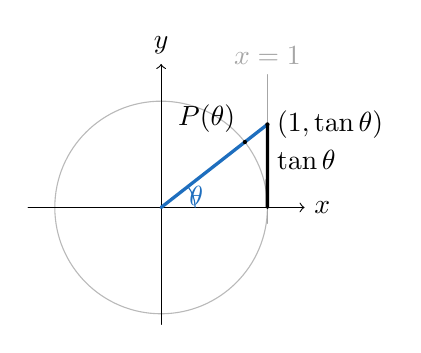
\begin{tikzpicture}[scale=1.35, line cap=round, line join=round]
  \definecolor{trigblue}{RGB}{30,110,190}
  \coordinate (O) at (0,0);
  \coordinate (P) at (38:1);
  \coordinate (T) at (1,{tan(38)});
  \draw[gray!55] (O) circle (1);
  \draw[->] (-1.25,0)--(1.35,0) node[right] {$x$};
  \draw[->] (0,-1.1)--(0,1.35) node[above] {$y$};
  \draw[gray!70] (1,-0.15)--(1,1.25) node[above] {$x=1$};
  \draw[very thick, trigblue] (O)--(T);
  \draw[very thick] (1,0)--(T);
  \fill (P) circle (0.02) node[above left] {$P(\theta)$};
  \fill (T) circle (0.02) node[right] {$(1,\tan\theta)$};
  \node[right] at (1,0.45) {$\tan\theta$};
  \draw[trigblue] (0.32,0) arc[start angle=0,end angle=38,radius=0.32];
  \node[trigblue] at (0.33,0.11) {$\theta$};
\end{tikzpicture}
\end{center}


\begin{definitionbox}{Definition}
\begin{definition}[Extended tangent]
\label{def:extended-tangent}
Where $\cos\theta\neq 0$, define
\[
  \tan\theta=\frac{\sin\theta}{\cos\theta}.
\]
\end{definition}
\end{definitionbox}
\begin{remark*}[Geometric reading]
The tangent of $\theta$ is the signed height where the terminal ray meets the
vertical tangent line $x=1$.
\end{remark*}
